\begin{tikzpicture}

    % Draw the square
    \draw[thick] (0, 0) rectangle (4, 4);
    
    % Draw the diagonal
    \draw[thick] (0, 0) -- (4, 4);

    \draw[thick, ->] (1.5,-0.5) -- (0, -0.5); 
    \draw[thick, ->] (2.5, -0.5) -- (4, -0.5);
    \node at (2,-0.5) {m};

    % Add red points at regular intervals along the diagonal
    \foreach \i in {0, 0.5, 1, 1.5, 2, 2.5, 3, 3.5, 4} {
        \fill[red] (\i, \i) circle (2pt);
    }

    \node[draw, fill=blue!20, text width=6cm, rounded corners] at (8, 4) {

        $\xrightarrow{} $ The slope of the line created by the change of the position of points is 1
    };

    \node[draw, fill=blue!20, text width=6cm, rounded corners] at (8, 1) {
    
        $\xrightarrow{} $ There are $m$ possible positions for a point in a cell for partition transition, each of them are consecutively spaced by $\sqrt{2}$ unit
    };   

     
    

\end{tikzpicture}